La presente distribuzione della materia risulta essere altamente disomogenea: si definiscono 
\textit{strutture cosmiche} i colossali ammassi (\textit{cluster}) di galassie tenuti insieme dalla
interazione gravitazionale tra i propri componenti, che raggiungono masse complessive tra $10^{13}$
e $10^{16}$ masse solari. Inoltre esistono sovrastrutture ancora più mastodontiche, dette superammassi.
I superammassi si presentano come un intricato reticolo di filamenti luminosi di galassie, che delimitano
spazi scuri, vuoti. Il fenomeno è noto come \textit{caustiche} e non ha solo applicazione in cosmologia, ma 
risulta trasversale in molteplici situazioni naturali. Il nome caustica si riferisce anche alla scomposizione
della luce sul fondo di una piscina, che ricorda in effetti le distribuzioni galattiche.

\begin{center}
	\begin{figure}[H]
		\centering
		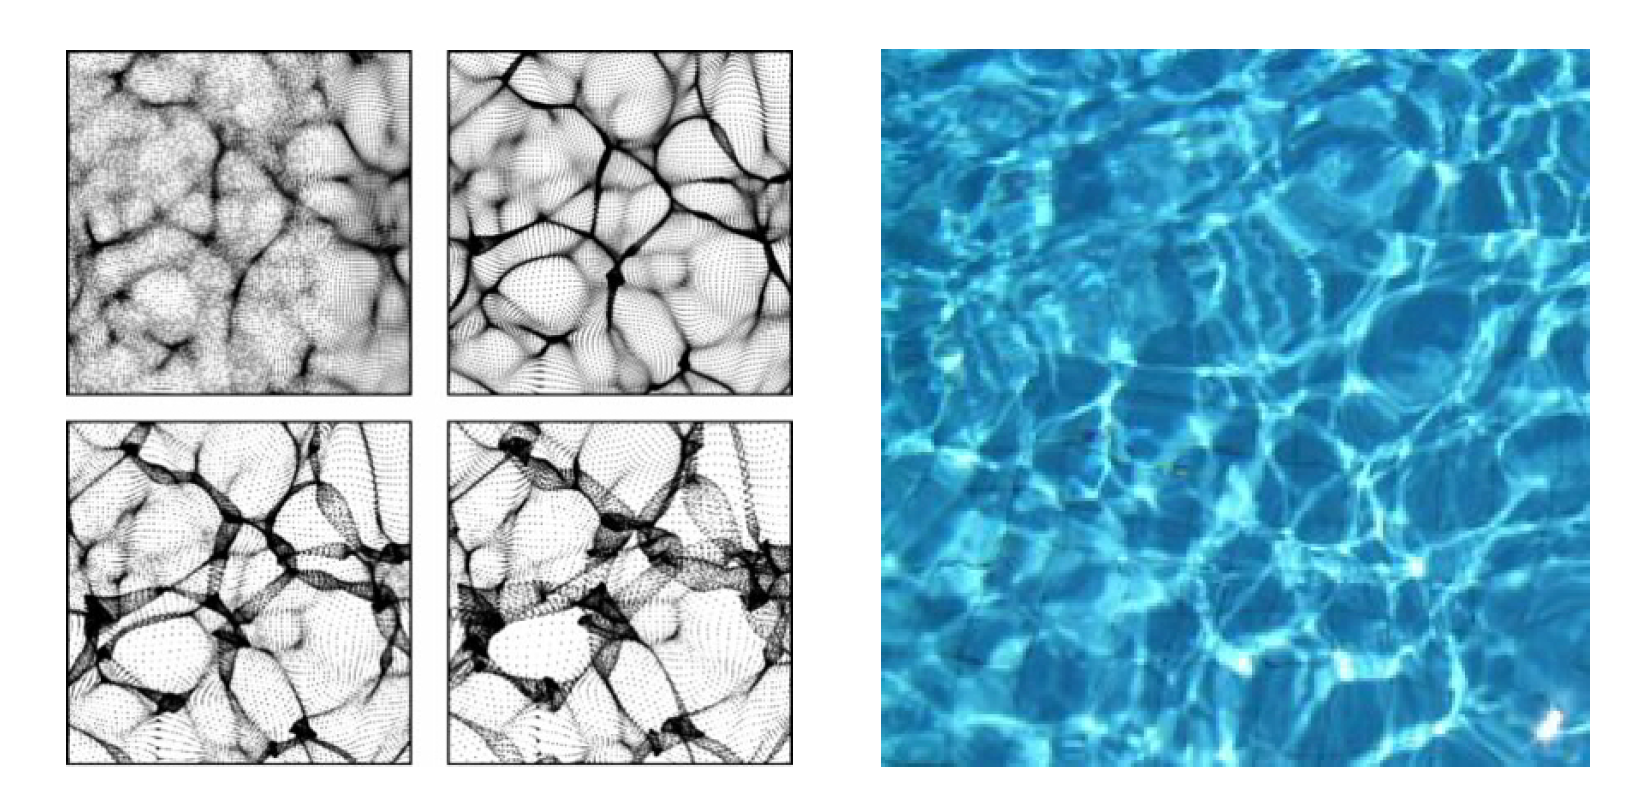
\includegraphics[scale=0.3, angle=0]{caustica.png}
        \caption{A sinistra, simulazione a N corpi bidimensionale fatta in approssimazione di Zel'dovich per crescenti
        oscillazioni di densità rispetto alla media $\rho_b$. A destra, caustica sul fondo di un piscina. Immagine tratta da \cite{gurbatov}.}
		\label{fig:caustica}
	\end{figure}
\end{center}

Questa distribuzione grumosa della massa si può descrivere con preciso approccio matematico, discusso nel primo capitolo,
e riguarda la teoria del \textit{trasporto ottimo}, che affronta proprio il problema di determinare il processo massimamente
efficiente, ovvero con il minimo dispendio, attraverso cui si può trasportare una certa distribuzione di massa iniziale a una 
finale.

